\UseRawInputEncoding
\documentclass[12pt]{article}
\usepackage[utf8]{inputenc}
\usepackage[spanish, es-tabla]{babel}
\usepackage{float}
\usepackage{indentfirst}
\usepackage{colortbl}
\usepackage{wrapfig}
\usepackage{csvsimple}
\usepackage[normalem]{ulem}
\usepackage{caption}
\usepackage{subcaption}
\usepackage{vmargin}
\usepackage{multirow}
\usepackage{amsmath}
\usepackage{mathrsfs}
\usepackage{enumitem}
\usepackage{amsfonts}
\usepackage{hyperref}
\usepackage{hhline}
\usepackage{tikz}
\usepackage{xcolor}
\usepackage{listings}
\usepackage{graphicx} 
\usepackage{amsmath}
\usepackage{amsfonts}
\usepackage{amssymb}
\usepackage{fancyvrb}
\usepackage{times}
\usepackage{hyperref}

\newcommand{\keyword}[1]{\textcolor{blue}{\textbf{#1}}}


\setpapersize{A4}
\setmargins{2.5cm}      % margen izquierdo
{1.5cm}                 % margen superior
{16.5cm}                % anchura del texto
{23.42cm}               % altura del texto
{10pt}                  % altura de los encabezados
{1cm}                   % espacio entre el texto y los encabezados
{0pt}                   % altura del pie de página
{2cm}

\setlength{\parindent}{2em}
\setlength{\parskip}{1em}

\usepackage{titlesec}

\titleclass{\subsubsubsection}{straight}[\subsection]

\newcounter{subsubsubsection}[subsubsection]
\renewcommand\thesubsubsubsection{\thesubsubsection.\arabic{subsubsubsection}}
\renewcommand\theparagraph{\thesubsubsubsection.\arabic{paragraph}} % optional; useful if paragraphs are to be numbered

\titleformat{\subsubsubsection}
  {\normalfont\normalsize\bfseries}{\thesubsubsubsection}{1em}{}
\titlespacing*{\subsubsubsection}
{0pt}{3.25ex plus 1ex minus .2ex}{1.5ex plus .2ex}

\makeatletter
\renewcommand\paragraph{\@startsection{paragraph}{5}{\z@}%
  {3.25ex \@plus1ex \@minus.2ex}%
  {-1em}%
  {\normalfont\normalsize\bfseries}}
\renewcommand\subparagraph{\@startsection{subparagraph}{6}{\parindent}%
  {3.25ex \@plus1ex \@minus .2ex}%
  {-1em}%
  {\normalfont\normalsize\bfseries}}
\def\toclevel@subsubsubsection{4}
\def\toclevel@paragraph{5}
\def\toclevel@subparagraph{6}
\def\l@subsubsubsection{\@dottedtocline{4}{7em}{4em}}
\def\l@paragraph{\@dottedtocline{5}{10em}{5em}}
\def\l@subparagraph{\@dottedtocline{6}{14em}{6em}}
\makeatother

\setcounter{secnumdepth}{4}
\setcounter{tocdepth}{4}

\begin{document}

\begin{titlepage}
\begin{center}

{
\includegraphics[width=0.4\textwidth]{itba-1.png}\par}
\vspace{1cm}
{\bfseries\LARGE Instituto Tecnológico de Buenos Aires \par}
\vspace{0.5cm}
{\scshape\Huge\underline {T.P. 2: Autómatas celulares} \par}
\vspace{0.4cm}
{\Large\itshape 72.25 - Simulación de Sistemas  \par}
\end{center}
\vfill

{\Large Integrantes \par}
\centering
{\Large Tepedino, Cristian - 62830 \par}
{\Large Bloise, Luca - 63004 \par}
{\Large Arias, Uriel Ángel - 63504 \par}

\vfill
{\Large\itshape Primer Cuatrimestre del 2025 \par}
\end{titlepage}

\setcounter{page}{0}
\tableofcontents
\clearpage

\section{Introducción}
En el siguiente informe se mostrarán los resultados de simular un modelo de Ising bidimensional para representar la opinión de un grupo de diferentes personas a través del tiempo en función de diferentes condiciones iniciales.

\section{Modelo de Ising}
El modelo de Ising es una red de spines que pueden apuntar hacia arriba o
hacia abajo. La red puede tener cualquier número de dimensiones y puede ser
de cualquier tipo (cuadrada, hexagonal, etc.). En este caso, al ser cuadrada se cuenta con una grilla de dimensión $N$ donde cada spin viene a representar la opinión particular de una persona. De esta manera, dada una configuración inicial de opiniones y una probabilidad de cambio de estado oponiéndose a la opinión de la mayoría, se puede calcular el cambio de estado de cada individuo luego de verificar el estado de sus vecinos adyacentes. Para esto se sigue el siguiente algoritmo:

Considerando una Grilla cuadrada de N x N (Con Condiciones Periódicas de Contorno).
Cada Sitio representa un individuo con dos posibles $S_{ij}\pm1$

Evolución:

- Elegir un sitio (i. j) al azar.
- Calcular el signo de la suma de los 4 vecinos: $$sign(S_{i-1 j}\!+\!S_{i+1j}\!+\!S_{i j-1}\!+\!S_{i j+1})$$

    - Si es distinto de cero, entonces la opinión de la mayoría es:
$$O_{M}=sign(S_{i-1 j}\!+\!S_{i+1j}\!+\!S_{i j-1}\!+\!S_{i j+1})$$

    - Sino:
$$O_{M}=S_{ij}$$

- Con probabilidad (1-p) adoptar el estado de la mayoría: $$S\space^\prime_{ij}=O_{M}$$

- Con probabilidad p cambiar el estado del Sitio: $$S\space^\prime_{ij}=-S_{ij}$$


Este proceso se repite considerando un periodo elegido, que en particular para este trabajo fue el de un paso de Montecarlo que corresponde a $N^{2}$ actualizaciones individuales.

A partir de la recolección de los estados obtenidos, luego de una cantidad de pasos considerable, es posible tomar métricas que reflejen los cambios producidos, dentro de las cuales se encuentran el consenso y la susceptibilidad.

El consenso se define formalmente como:
    $$M(t)=|{\frac{1}{N^{2}}}\sum_{i,j}S_{i,j}(t)|$$ (1)

La susceptibilidad se define formalmente como:
    $$\chi=N^{2}\left(\langle M^{2}\rangle-\langle M\rangle^{2}\right)$$ (2)

\section{Implementación}
\begin{figure}[h]
    \centering
    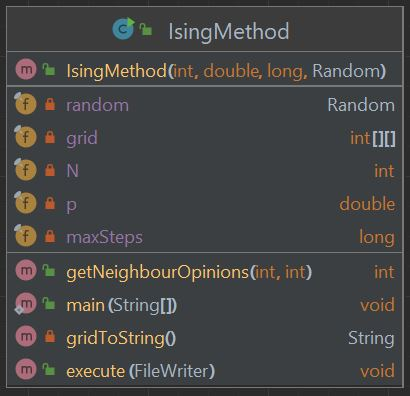
\includegraphics[width=0.6\textwidth]{uml_ising_method.JPG} 
    \caption{Diagrama UML para la clase IsingMethod}
    \label{fig:example}
\end{figure}

\subsection{Condiciones Iniciales}
Para poder realizar múltiples simulaciones con condiciones iniciales distintas se realizó una implementación parametrizada por medio de las propiedades del sistema que están disponibles en Java. De este modo, se pueden pasar los valores correspondientes a las siguientes propiedades: 'n' (referido como $N$ en el modelo), 'p', 'mcSteps' (número de pasos de Montecarlo a completar), 'seed' (valor utilizado para inicializar la clase que se encarga de generar números pseudoaleatorios para los pasos del proceso) y 'output' (nombre del archivo de salida con el resultado de la simulación). Resulta relevante aclarar que solo para los casos de 'n' y 'p' se requiere algún valor especificado, el resto de las propiedades son opcionales dado que por defecto se corre la simulación hasta que se envíe una señal para interrumpir al proceso, se usa una seed aleatoria desconocida y se escriben los resultados de la simulación en un archivo de nombre 'output.txt'.

Considerando que se utilizó una red cuadrada representada por medio de una matriz, o de forma más rigurosa, un arreglo de arreglos, se decidió inicializar las posiciones iniciales de la misma con valores pseudoaleatorios. Para esto, valiéndose de la implementación provista por la clase Random de java.util, se obtiene un valor booleano que se traduce en alguno de los dos valores posibles para cada posición. Este proceso se lleva a cabo dentro del constructor de la clase $IsingMethod$

\subsection{Evolución del modelo}
Habiendo definido la matriz inicial, se pone en marcha la simulación llamando al método $execute(FileWriter)$ que se encarga de ejecutar el algoritmo explicado en la sección anterior hasta la condición definida por los parámetros iniciales. A su vez, se encarga de imprimir el resultado de la simulación en un archivo de salida, el cual se inicia con los valores de los parámetros $N$, $p$ y $maxSteps$ junto con la matriz inicial que se imprime llamando al método $gridToString()$ de manera tal que cada fila se imprime en orden con todos los valores separados por un espacio en blanco.

A propósito de la implementación del algoritmo, el método $getNeighbourOpinions(int, int)$ se encarga de calcular la opinión de la mayoría de los vecinos para una celda especificada por medio del índice de fila y columna que se pasan por parámetro. En este método se tienen en cuenta las condiciones periódicas de contorno al momento de calcular cuáles son las posiciones que se requieren revisar como parte de las celdas vecinas. 

\subsection{Salida}
Luego de cada paso de Montecarlo se imprimen las posiciones de las celdas que cambiaron de estado respecto del paso anterior, indicándose en cada línea el índice de la fila y la columna de la celda. A continuación en una nueva línea se encuentra la palabra 'next' o 'end' que indica si hay o no un siguiente paso en la simulación ejecutada.

\section{Simulaciones}
\subsection{Variaciones del sistema con un $N$ fijo}
En primer lugar, se experimentó con un tamaño de $N = 50$ para la matriz inicial, de manera tal de ver que efectos se pueden observar de someter el sistema a diferentes valores de $p$: \{0.01, 0.1, 0.9\}. El objetivo de esta simulación es poder entender en que valores de p se obtiene una mayor variación de las opiniones en la grilla, a partir de lo que se puede observar de animar cada uno de los pasos realizados.

A continuación, tomando en cuenta, que una de las formas de medir el resultado de aplicar este modelo una cantidad finita de veces es por medio del consenso, se decidió tomar los mismos valores de $p$ pero considerando una cantidad de pasos suficiente para alcanzar un estado estacionario. Con esta simulación se pretende observar la variación del consenso hasta alcanzar el estacionario luego de un cierto número de pasos y poder comparar estos valores una vez alcanzado este valor. 

Luego, considerando los observables definidos anteriormente, se tomaron 10 valores de $p$ distintos para poder visualizar la variación del consenso y la susceptibilidad a lo largo de los diferentes valores elegidos en torno al $p_{critico}$. El objetivo de esta simulación consiste en poder analizar de forma más precisa la evolución del sistema ante diferentes valores de $p$, evidenciando el comportamiento del sistema al acercarse $p_{crítico}$.

\subsection{Variaciones del sistema con un $N$ variable}
Finalmente, se repite la última simulación descrita pero, en este caso, se busca tomar valores por debajo y por encima del $N$ fijado anteriormente. Los valores tomados para comparar son $N = \{25,50,75,100\}$. 
 
\section{Resultados}
\subsection{Variaciones del sistema con $N = 50$}
Para la primera simulación se decidieron realizar tres animaciones, una por cada valor de $p$ utilizado. Por otro lado para visualizar la evolución del consenso, se tomaron 30000 pasos de Montecarlo y se graficaron los valores obtenidos.

Para $p = 0.01$:

\begin{figure}[H]
    \centering
    \includegraphics[width=0.6\textwidth]{animación_0.01_50.png} 
    \caption{Fotograma de la animación de la simulación con p = 0.01 y N = 50}
\end{figure}

Para observar la animación utilizar el siguiente \href{https://www.youtube.com/watch?v=dQw4w9WgXcQ}{link a Youtube}

Por otro lado, para la evolución del consenso se obtuvo el siguiente gráfico:
\begin{figure}[H]
    \centering
    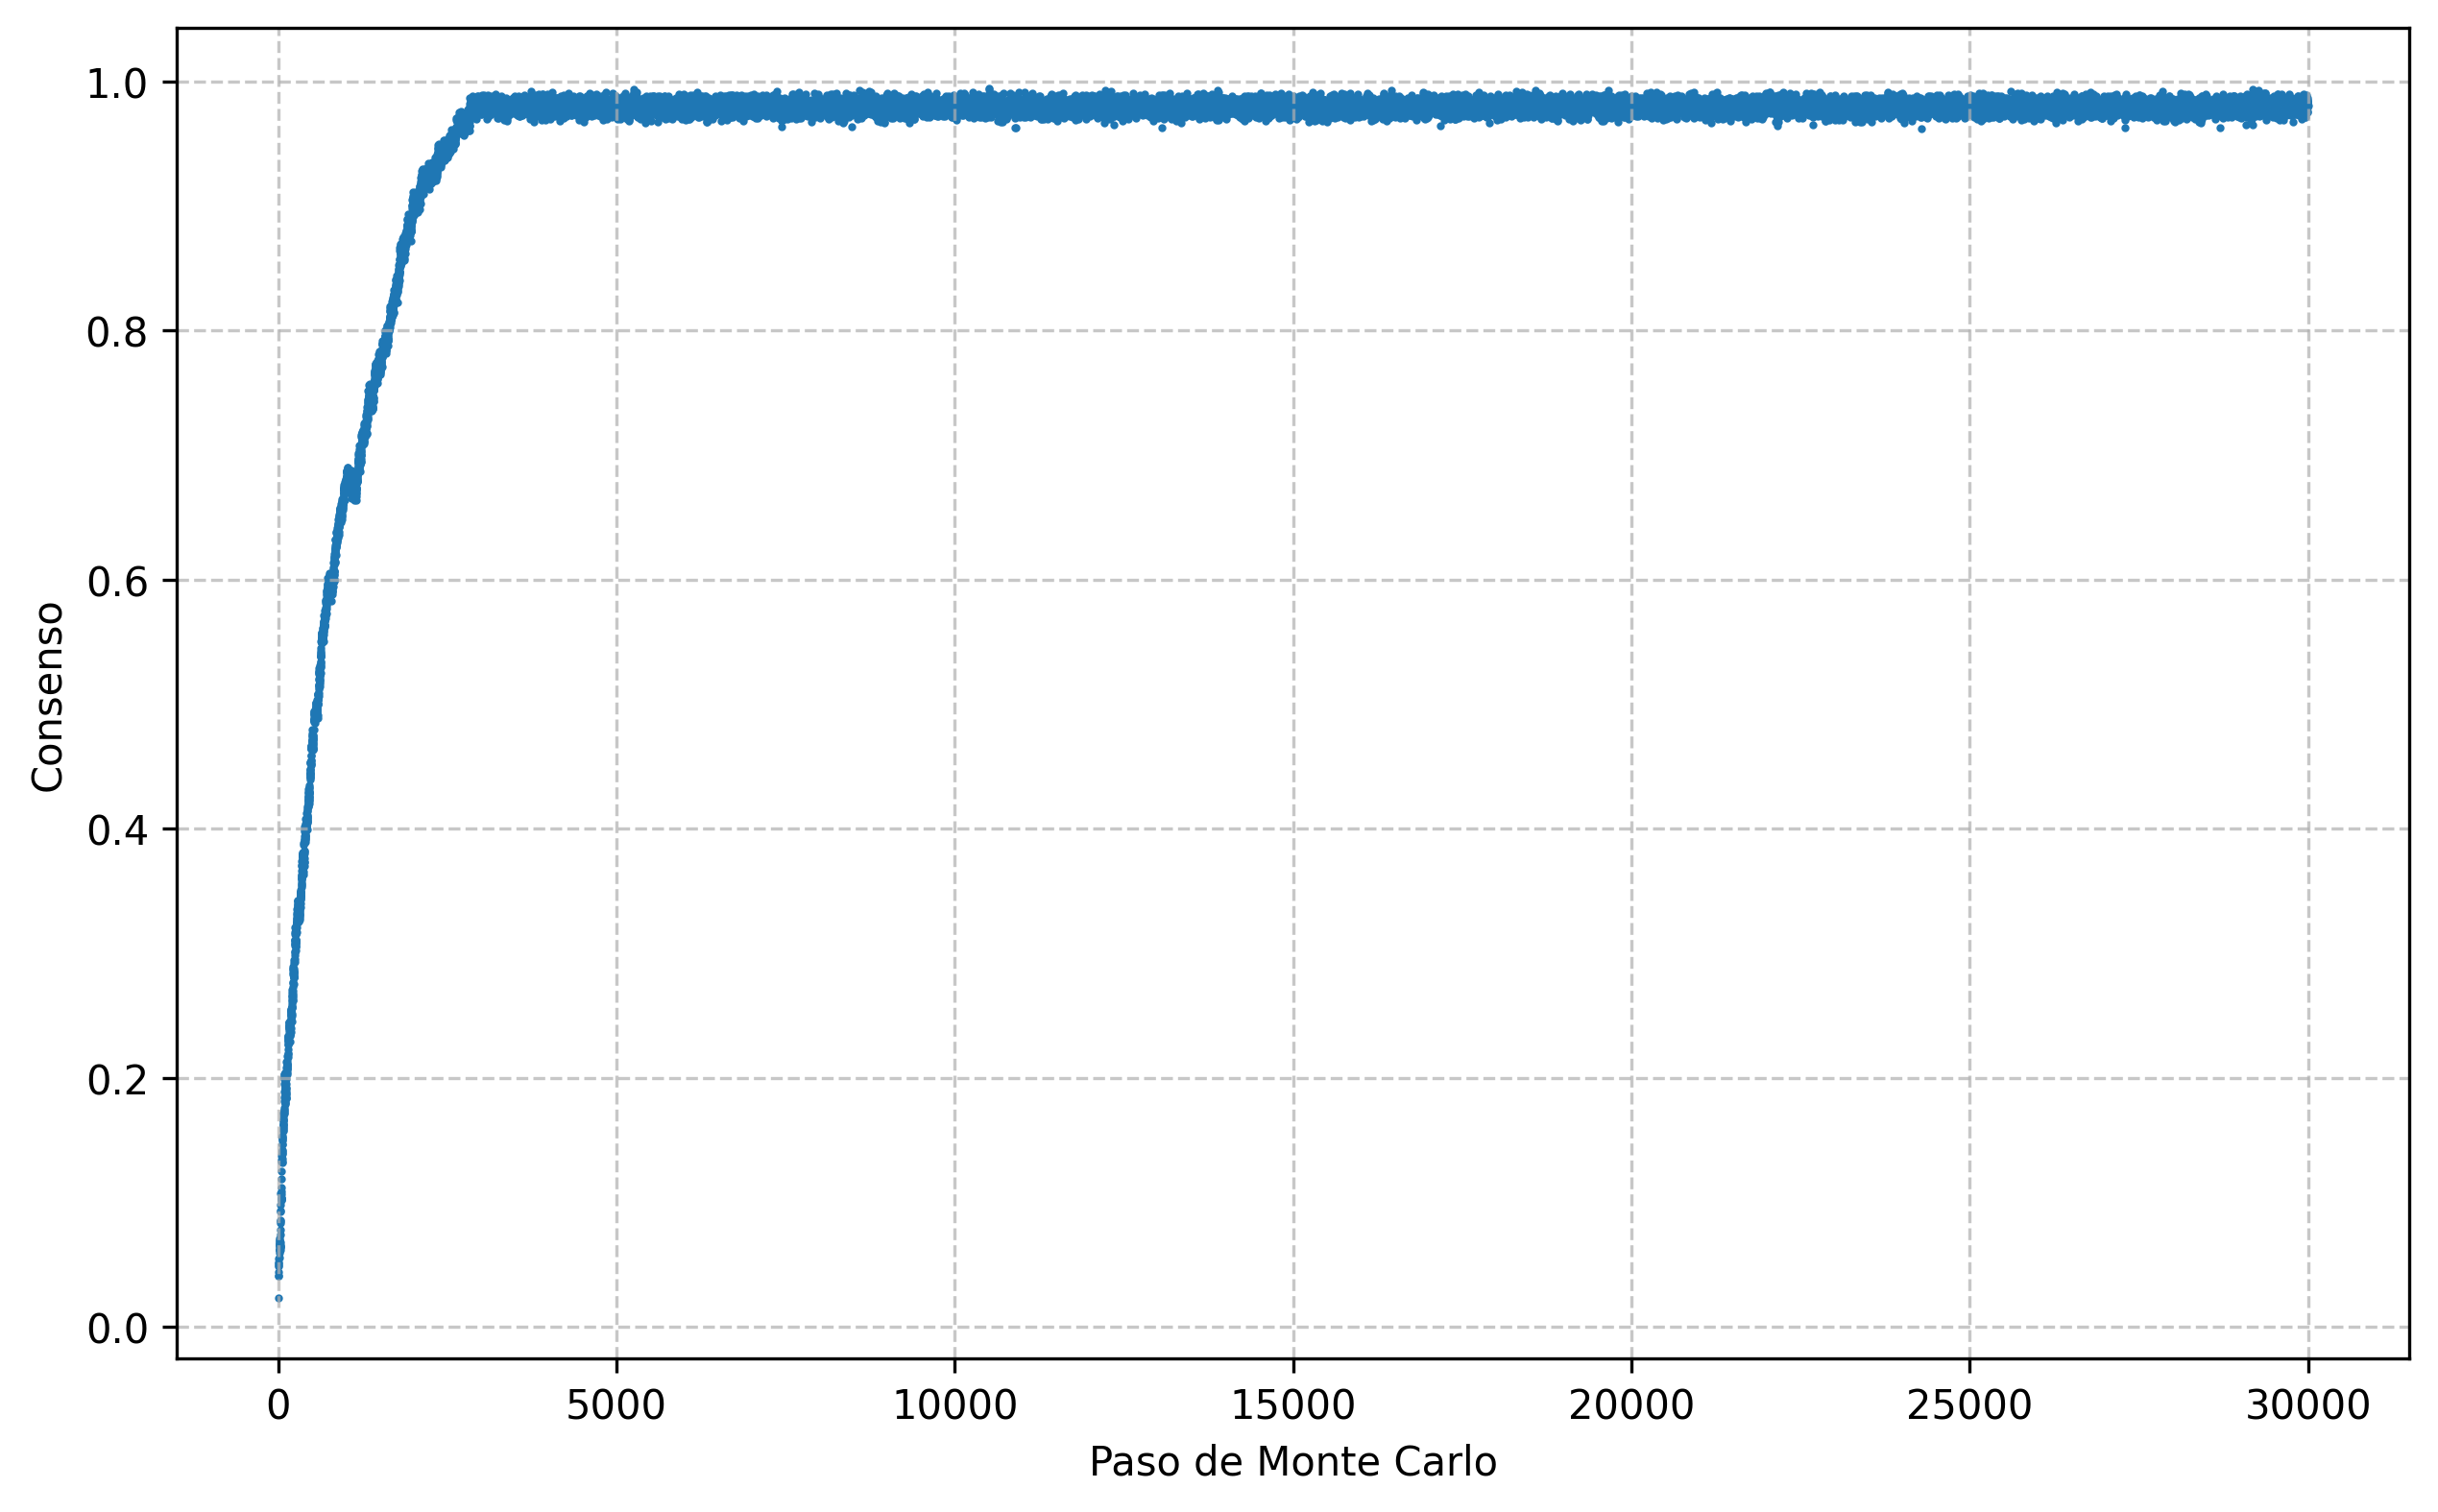
\includegraphics[width=1\textwidth]{consensus_evolution_n_50_p_0.01.png} 
    \caption{Consenso vs pasos de Montecarlo para p=0.01 y N=50}
\end{figure}

En este caso se puede observar como luego de menos de 5000 pasos se empieza a estabilizar el valor del consenso en un valor cercano por encima de 0.95. Esto se podría explicar teniendo en cuenta que se trata de un valor de p que favorece a que cada individuo tenga con una gran probabilidad la misma opinión que la mayoría de sus vecinos por lo que rápidamente se alcanza un grado de consenso elevado.

Para $p = 0.1$:

\begin{figure}[H]
    \centering
    \includegraphics[width=0.6\textwidth]{animación_0.1_50.png} 
    \caption{Fotograma de la animación de la simulación con p = 0.1 y N = 50}
\end{figure}

Para observar la animación utilizar el siguiente \href{https://www.youtube.com/watch?v=dQw4w9WgXcQ}{link a Youtube}

Por otro lado, para la evolución del consenso se obtuvo el siguiente gráfico:
\begin{figure}[H]
    \centering
    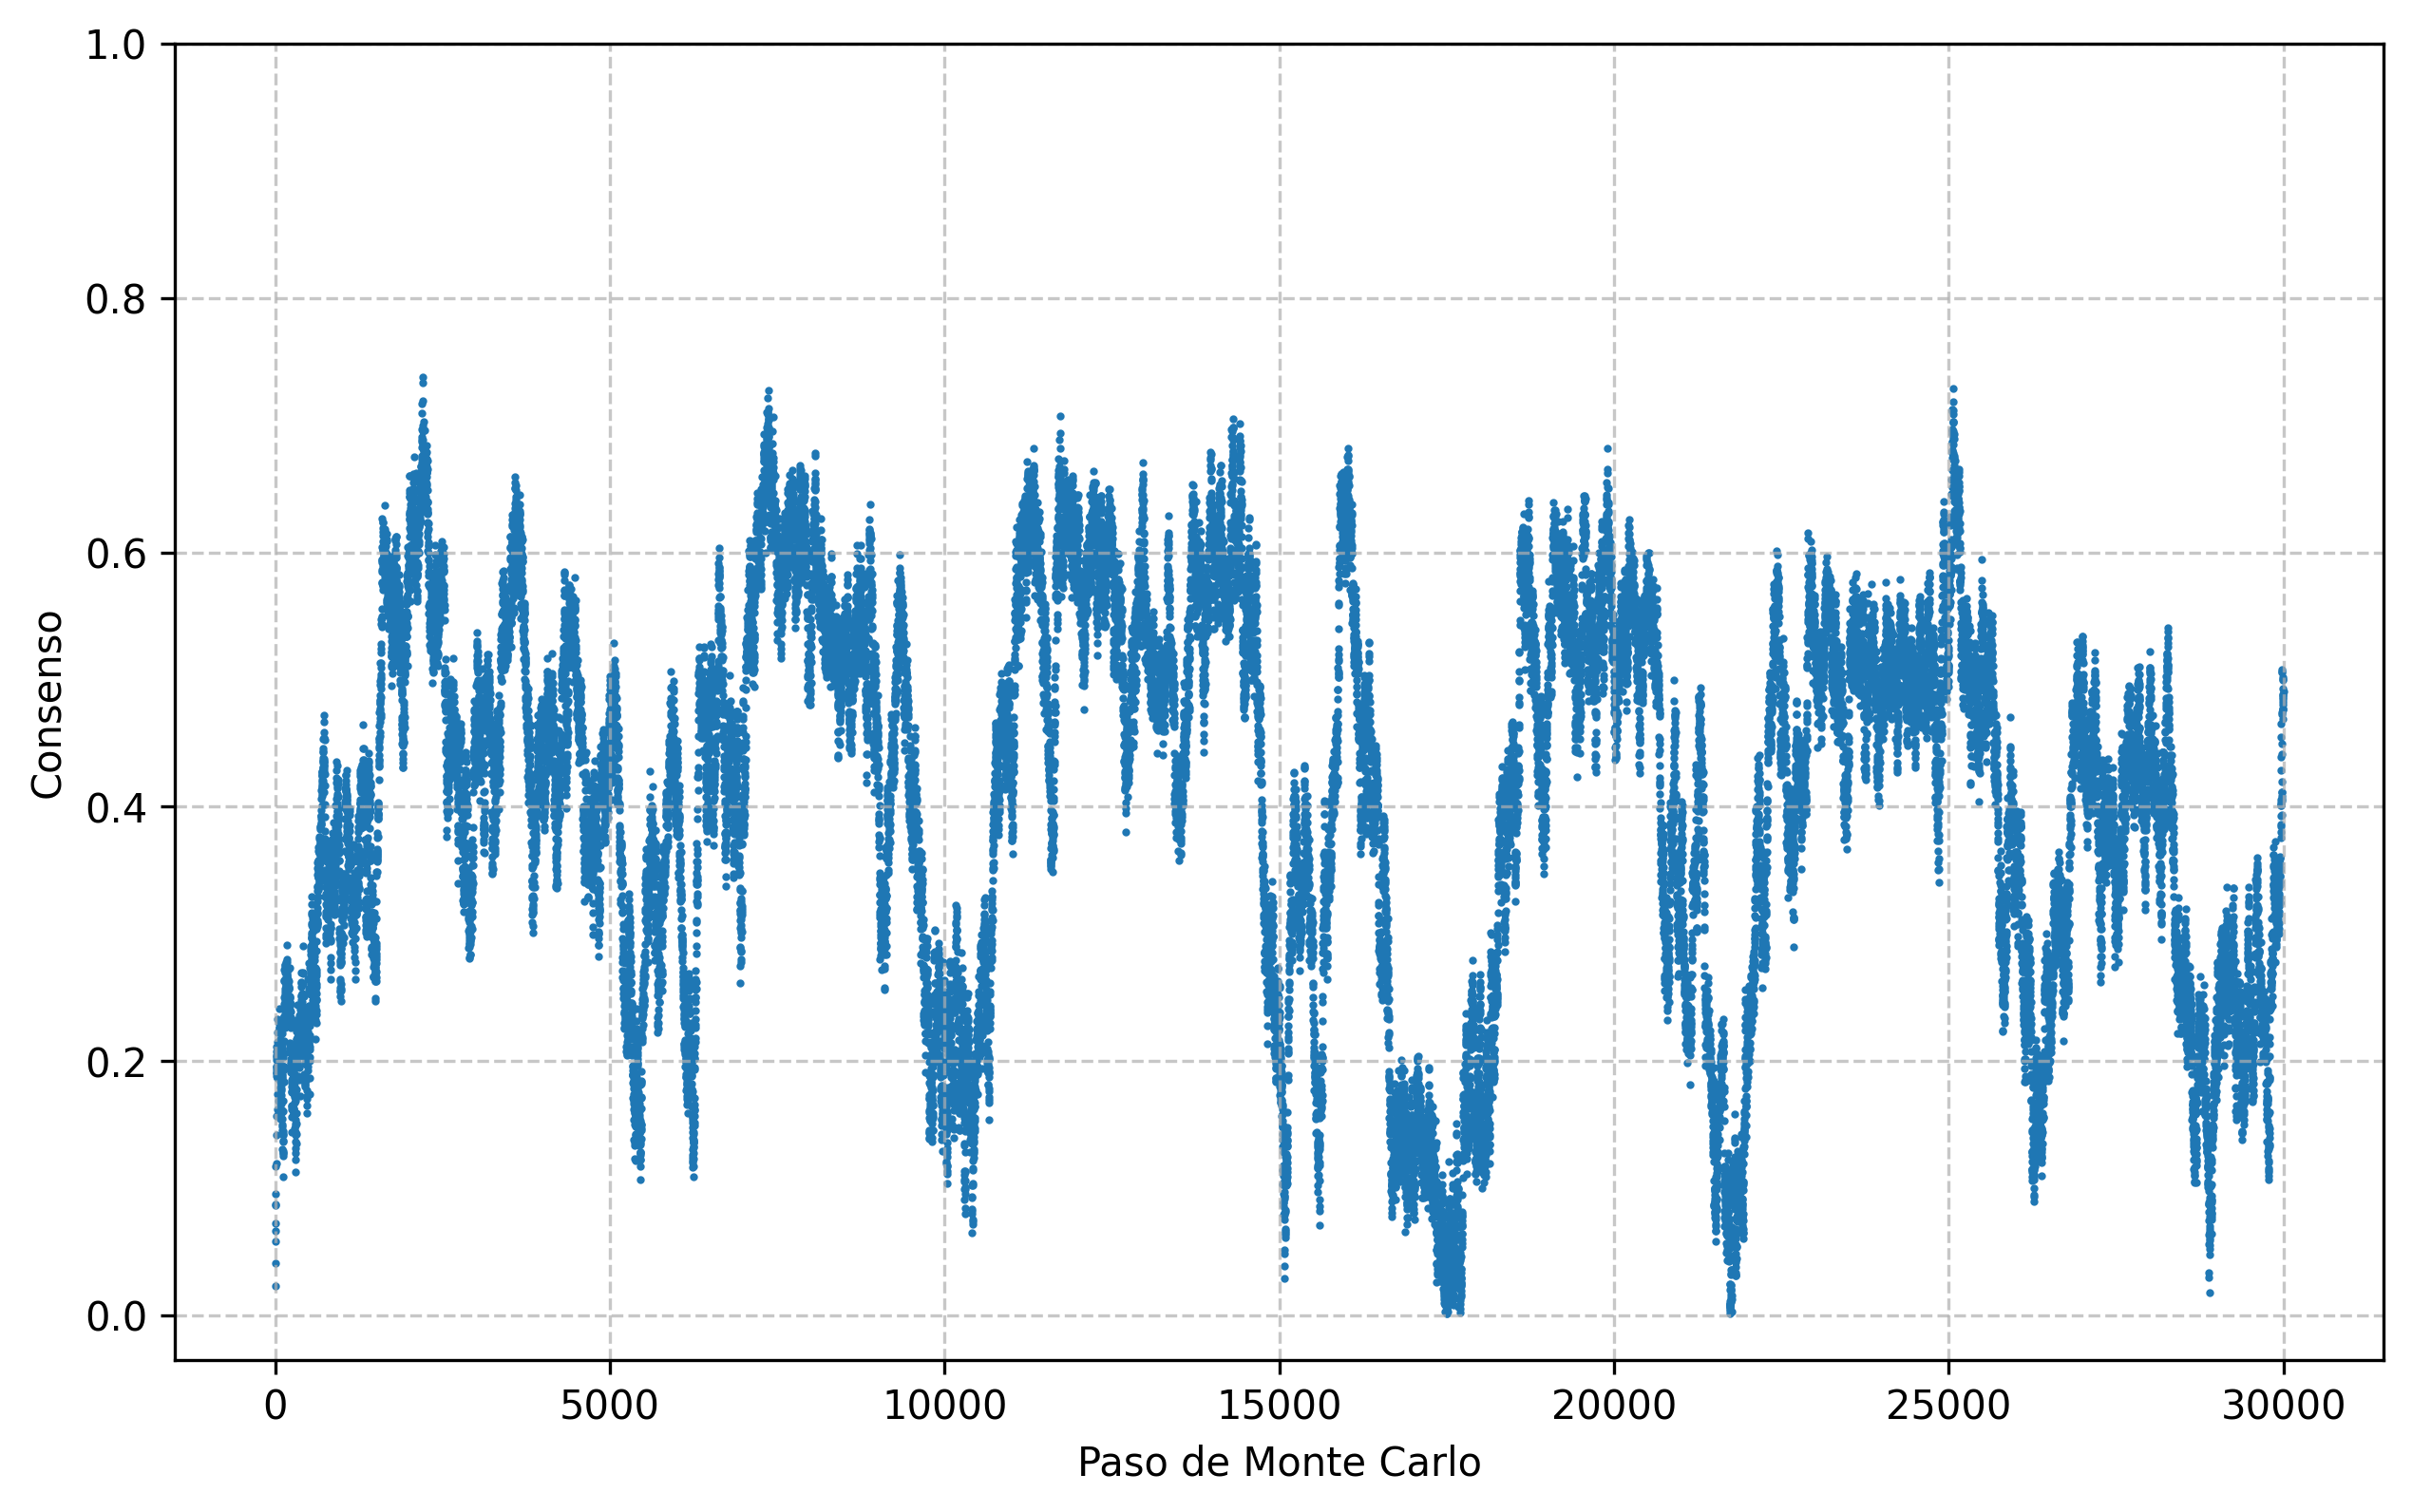
\includegraphics[width=1\textwidth]{consensus_evolution_n_50_p_0.1.png} 
    \caption{Consenso vs pasos de Montecarlo para p=0.1 y N=50}
\end{figure}

En este caso se puede observar como luego de una serie de pasos si bien se sigue teniendo un valor del consenso variable, se repiten los valores que oscilan desde 0.01 hasta 0.7 aproximadamente. 

Para $p = 0.9$:

\begin{figure}[H]
    \centering
    \includegraphics[width=0.6\textwidth]{animación_0.9_50.png} 
    \caption{Fotograma de la animación de la simulación con p = 0.9 y N = 50}
\end{figure}

Para observar la animación utilizar el siguiente \href{https://www.youtube.com/watch?v=dQw4w9WgXcQ}{link a Youtube}

\begin{figure}[H]
    \centering
    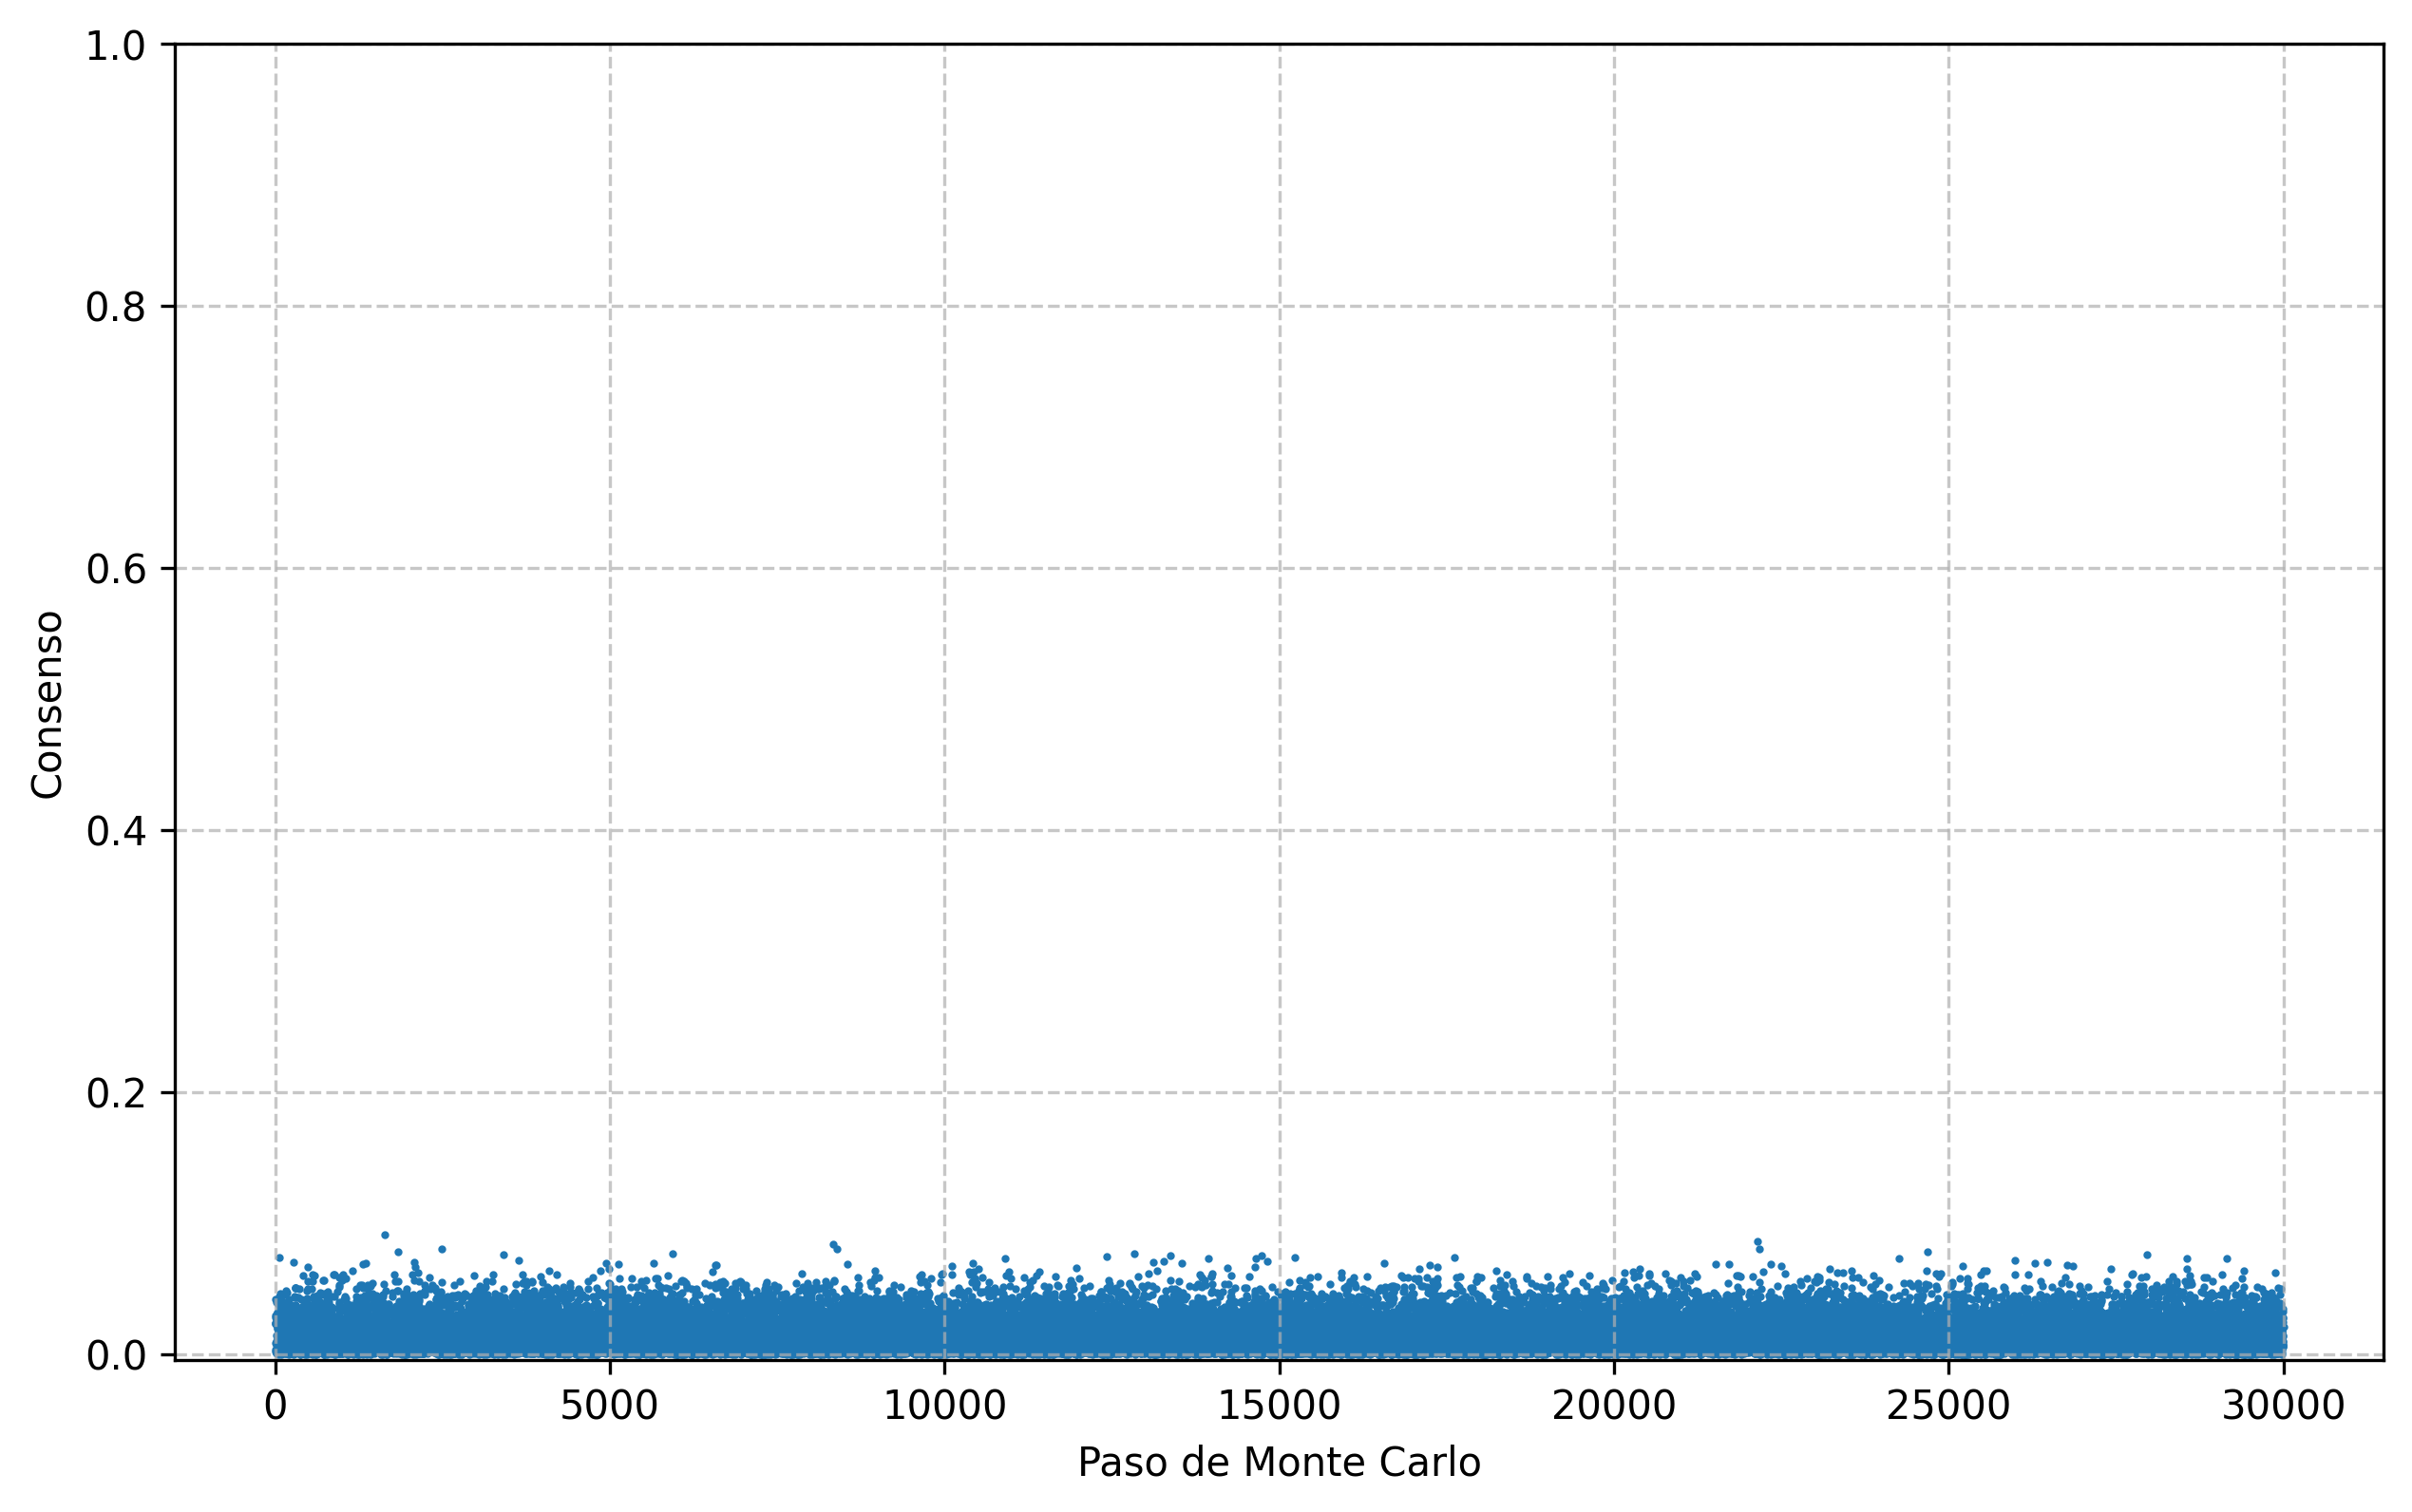
\includegraphics[width=1\textwidth]{consensus_evolution_n_50_p_0.9.png} 
    \caption{Consenso vs pasos de Montecarlo para p=0.9 y N=50}
\end{figure}

En este caso nuevamente se puede encontrar rápidamente una variación de valores aunque en este caso se agrupan principalmente por debajo de 0.1. Nuevamente es un resultado que acompaña con lo esperado considerado que se trata del valor más alto utilizado y lleva a que en la mayoría de los casos cada individuo vaya en contra de la opinión del resto de sus vecinos.

Por otro lado para las simulaciones que se realizaron con los 10 valores de p alrededor de $p_{critico}$. Para esto se realizaron una serie de pruebas preliminares tomando diferentes valores para validar el valor aproximado de $p_{crítico}$ considerando el comportamiento observado en la simulación anterior. Como resultado, se encontró el punto crítico en 0.1 y se tomaron los siguientes puntos para realizar las simulaciones:

$p = \{0.01, 0.05, 0.075, 0.0875, 0.09375, 0.096875, 0.10625, 0.1125, 0.125, 0.15, 0.2\}$

Para cada uno de ellos se decidieron hacer 10 simulaciones considerando diferentes seeds de manera tal de luego calcular un promedio a partir de los valores estacionarios obtenidos de cada una de ellas.

A continuación se presentan los resultados obtenidos para ambos observables:

\begin{figure}[H]
    \centering
    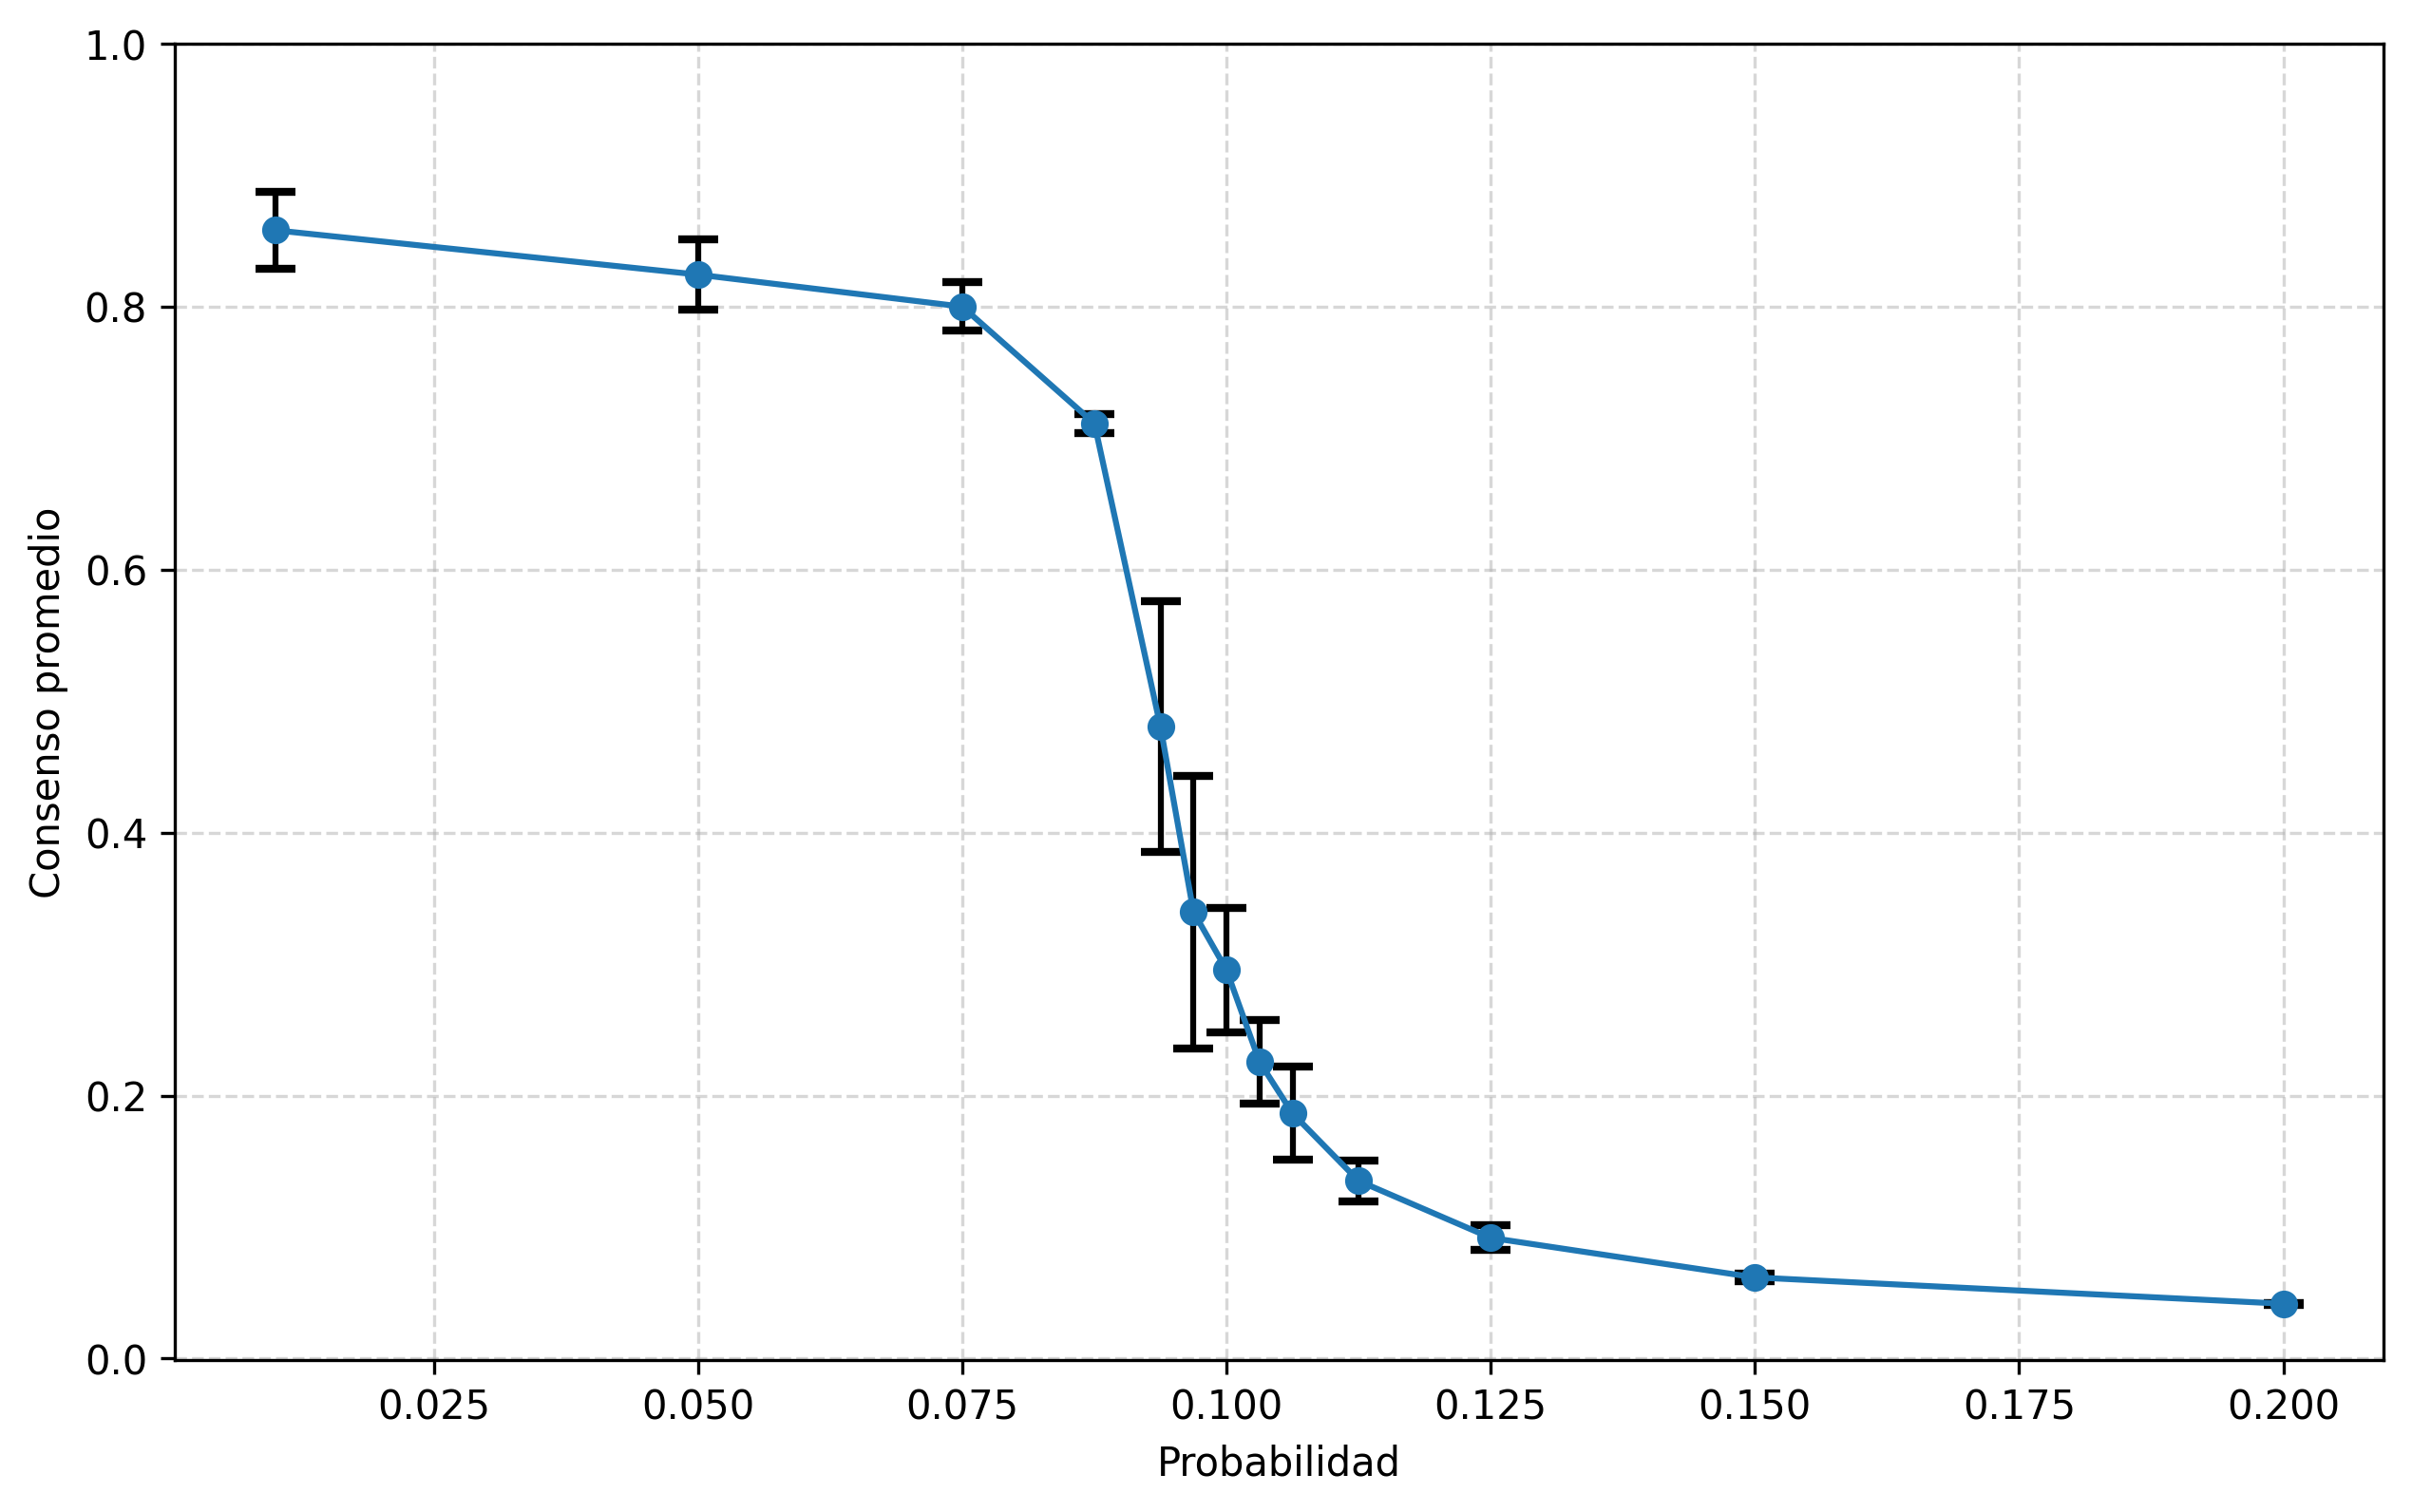
\includegraphics[width=1\textwidth]{magnetization_mean_n_50.png} 
    \caption{$\lt M\gt $ vs p}
\end{figure}

\begin{figure}[H]
    \centering
    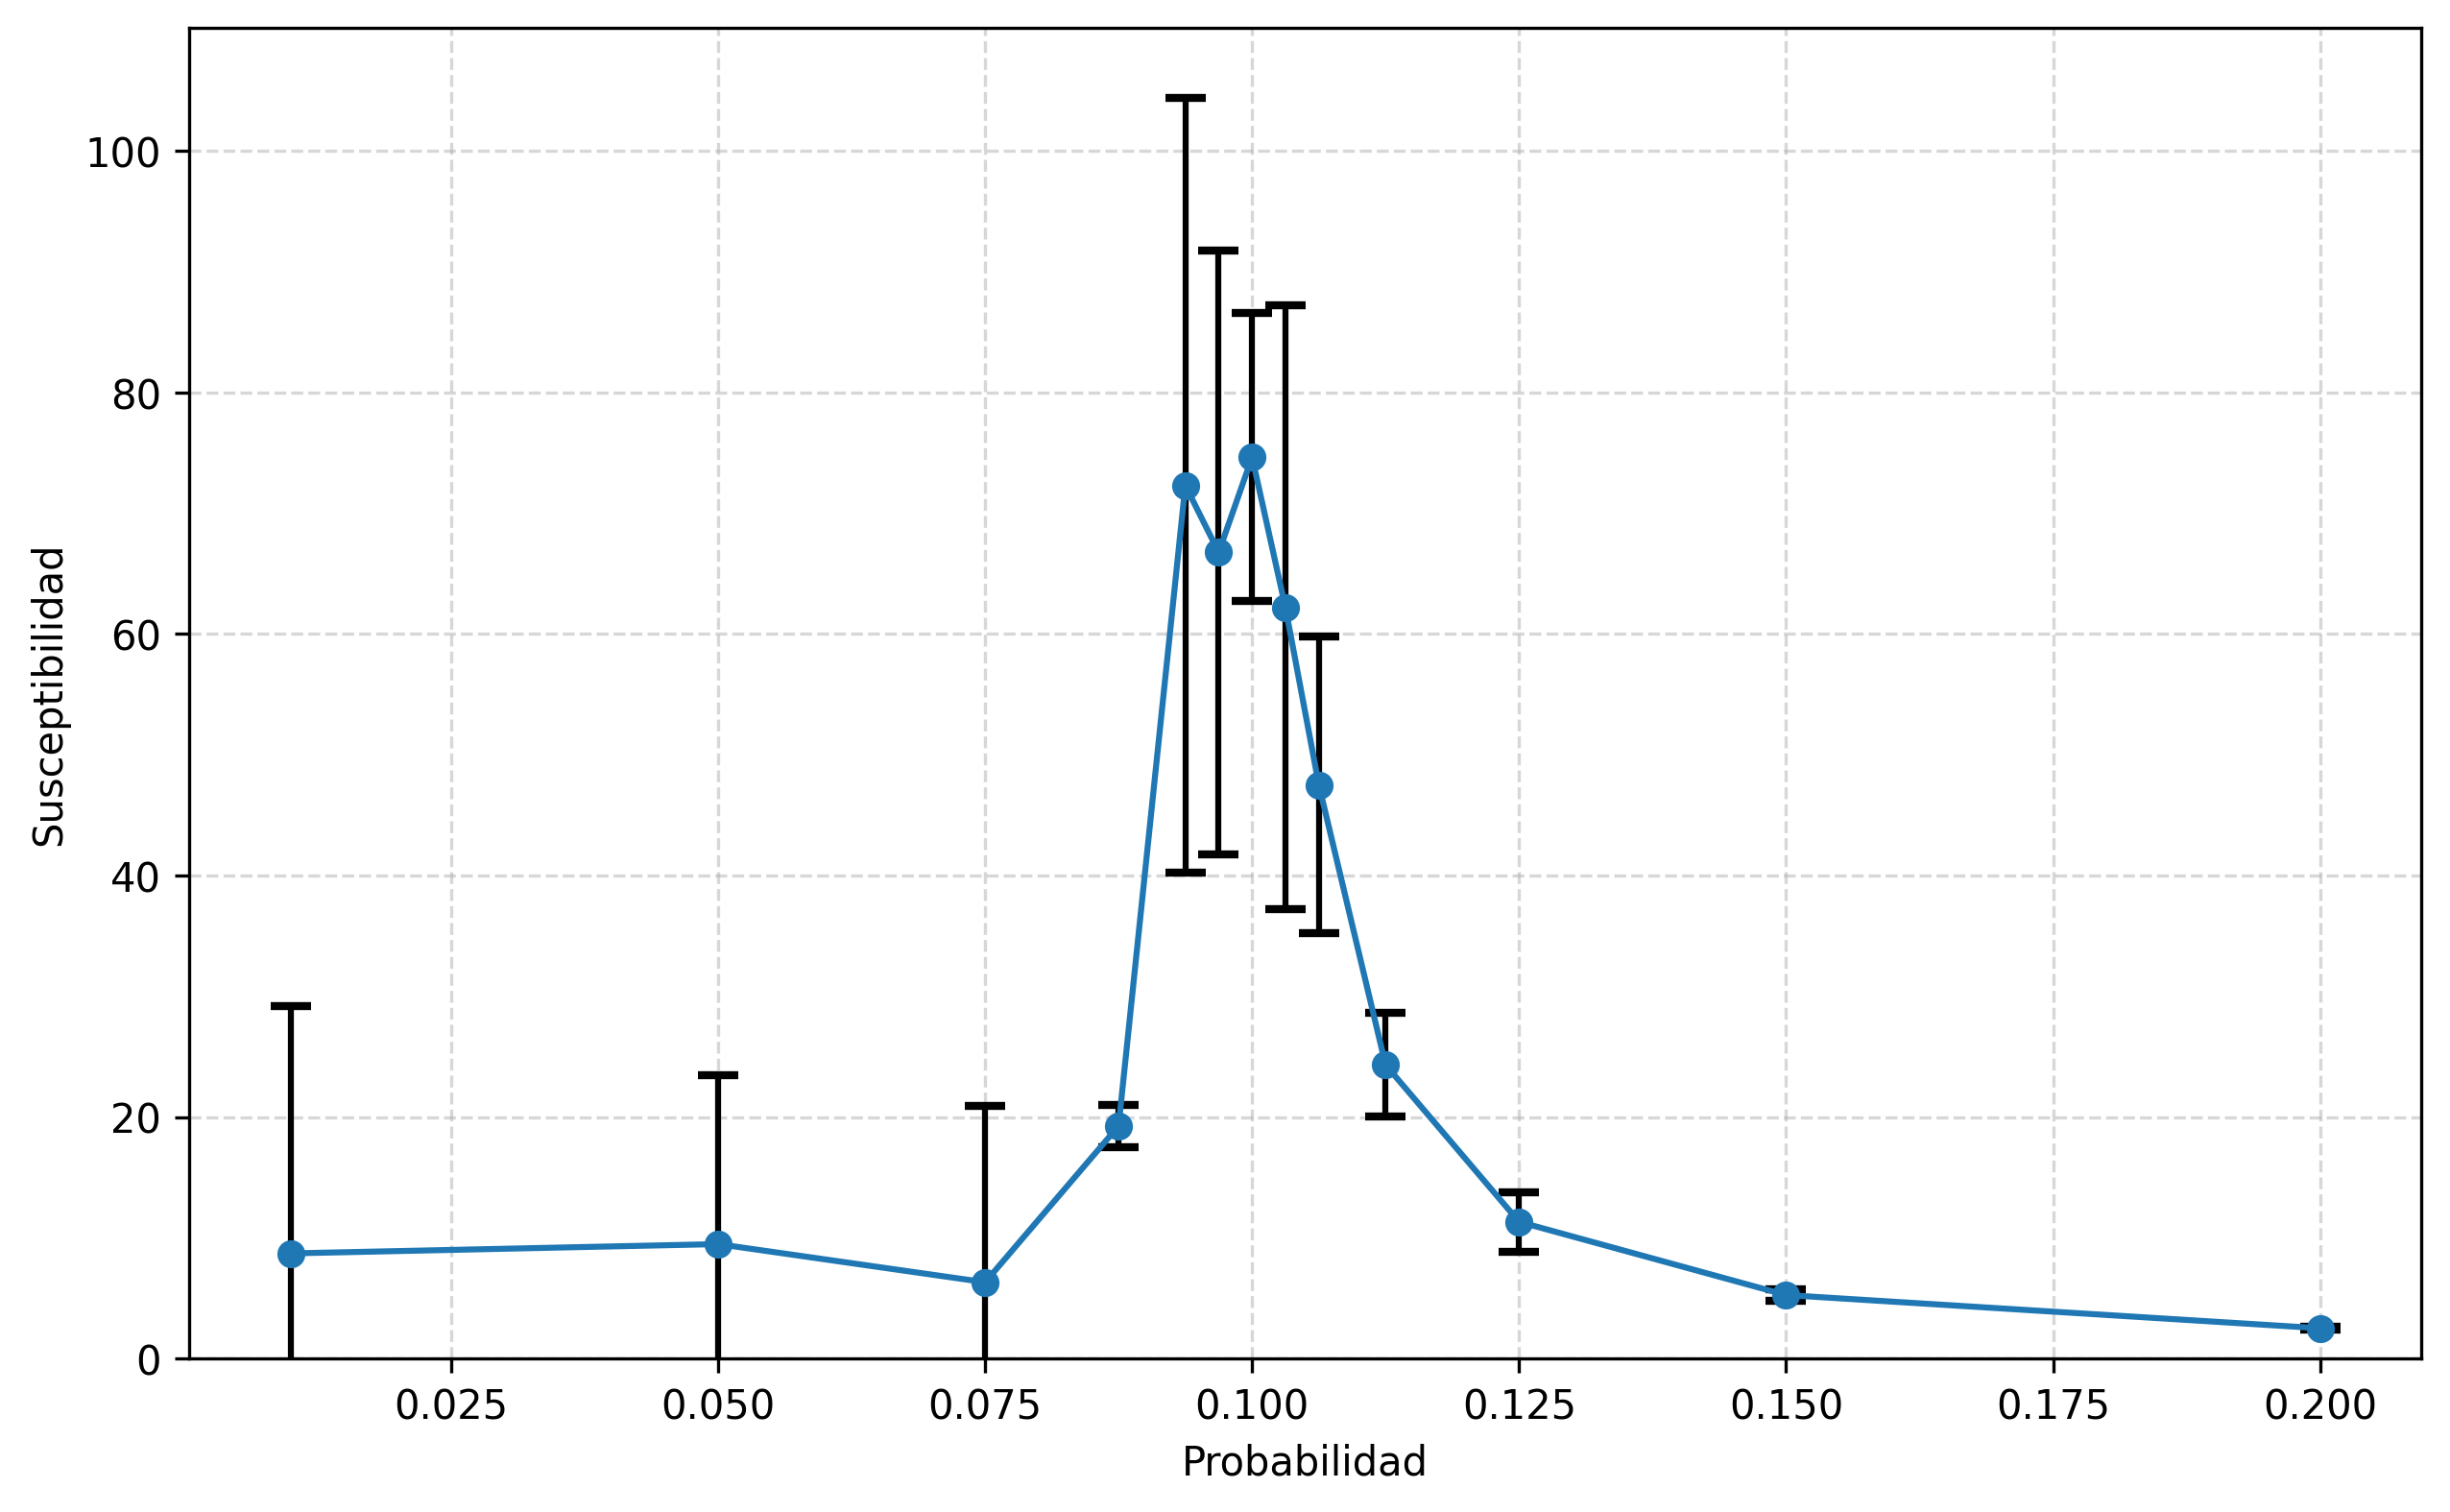
\includegraphics[width=1\textwidth]{susceptibility_50.png} 
    \caption{$\chi$ vs p}
\end{figure}

De estos gráficos se puede destacar como en los valores cercanos al $p_{critico}$, donde el consenso está en un estado transitorio por tener una pendiente más alta de descenso, se encuentran errores más altos. A su vez es en estos valores que se puede encontrar mayores valores de susceptibilidad, lo que concuerda con lo observado para el consenso.

\subsection{Variaciones del sistema con un $N$ variable}
Para esta simulación se decidieron tomar los valores de $N = \{25,75,100\}}$ los cuales se utilizaron para correr las simulaciones para cada una con la misma metodología que fue explicada para la simulación anterior.

Se decidió incluir en cada caso el resultado obtenido en $N = 50$ para que sea más simple la comparación de los resultados.

\begin{figure}[H]
    \centering
    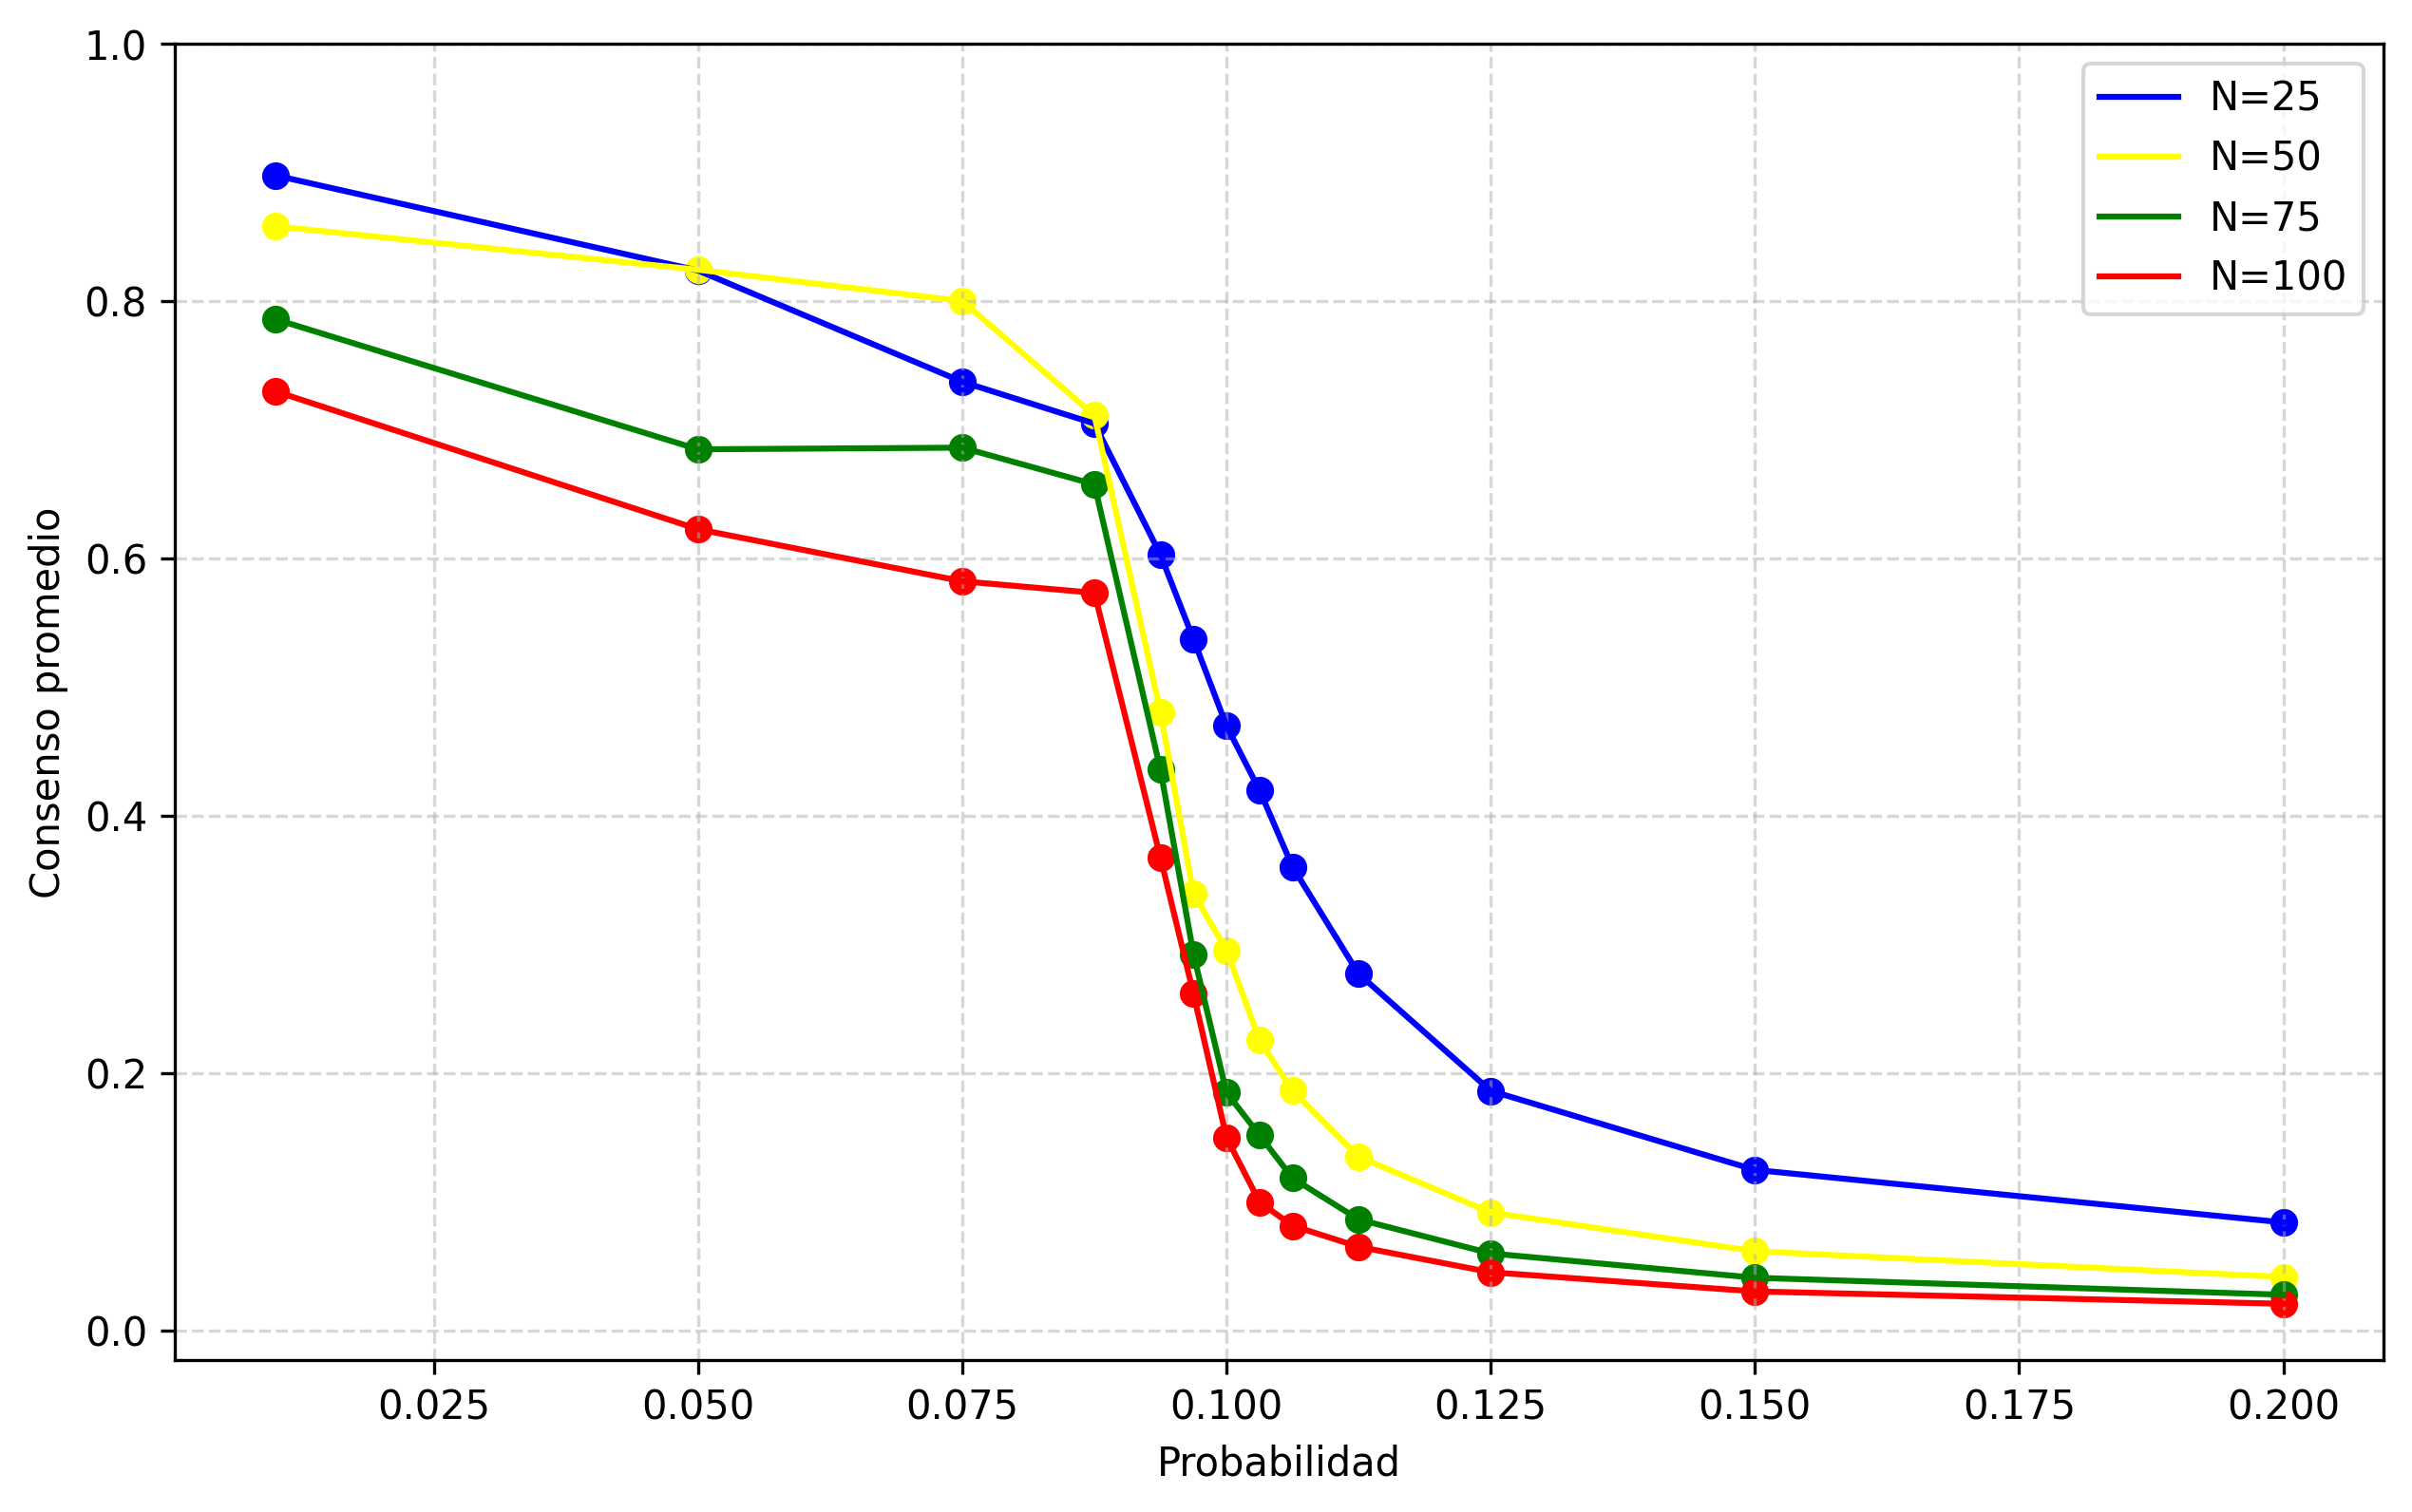
\includegraphics[width=1\textwidth]{magnetization_mean_comparison.png} 
    \caption{$\lt M\gt $ vs p}
\end{figure}

\begin{figure}[H]
    \centering
    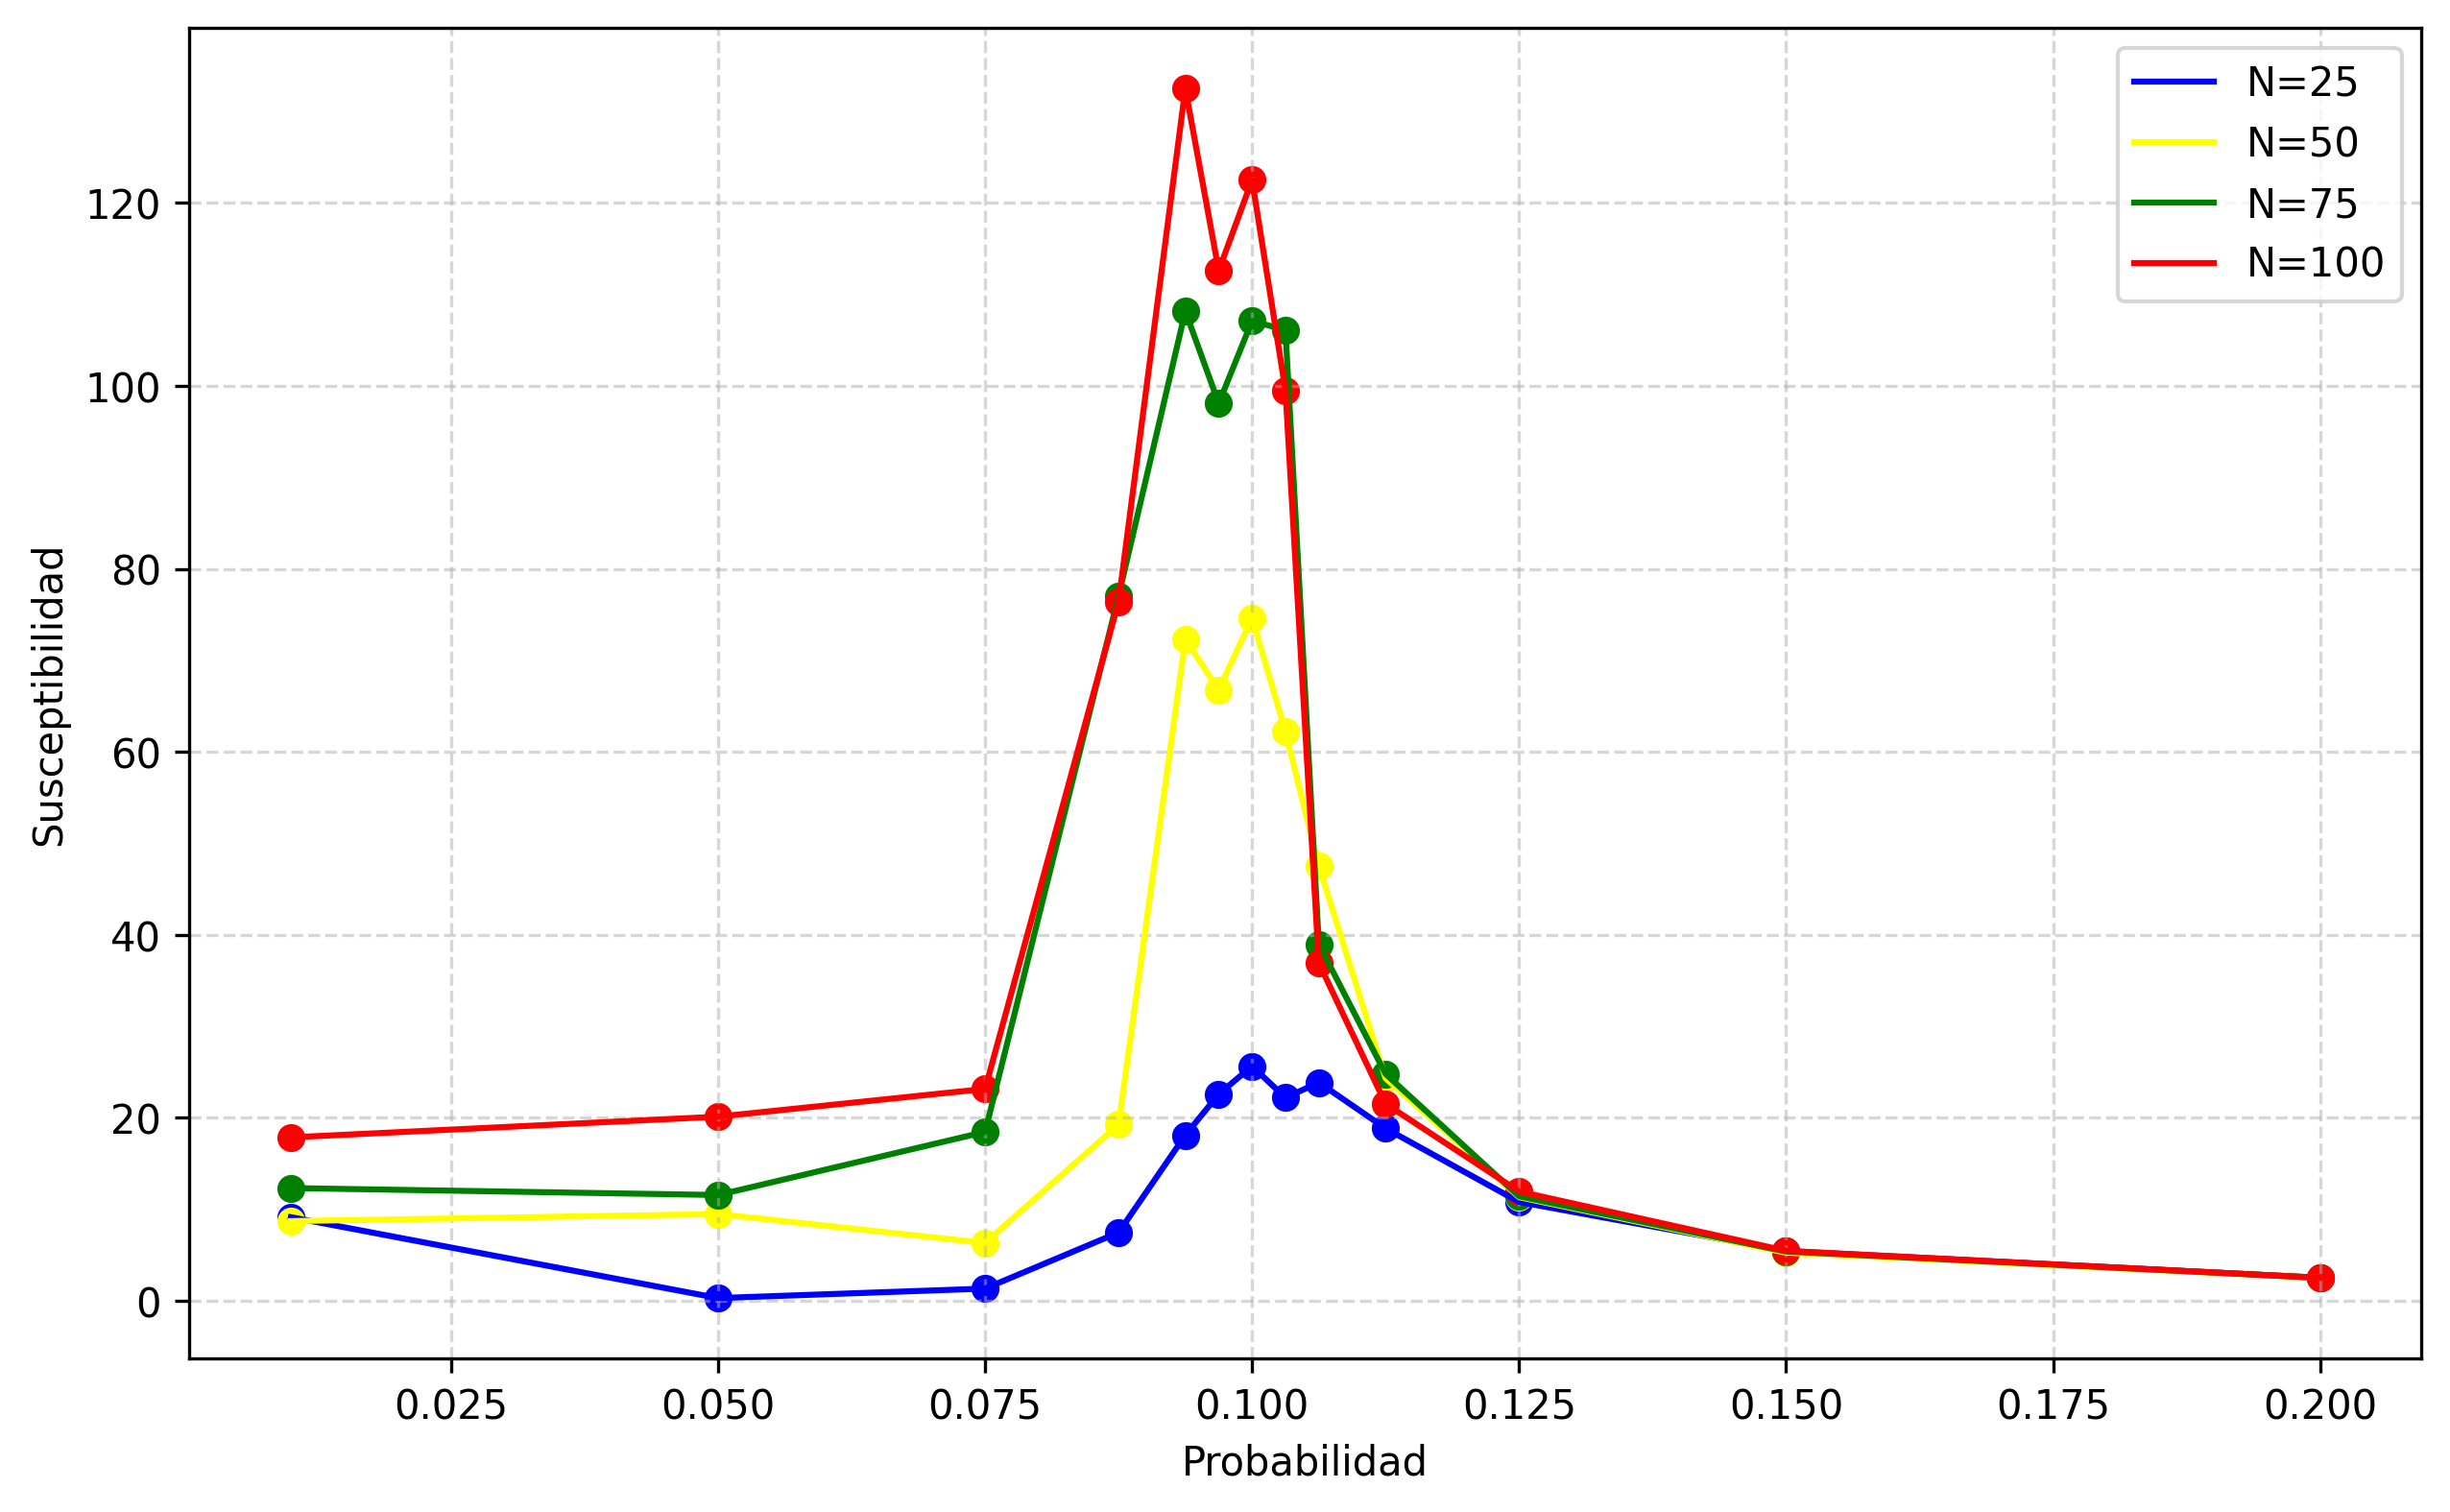
\includegraphics[width=1\textwidth]{susceptibilities_comparison.png} 
    \caption{$\chi$ vs p}
\end{figure}

A partir de estos resultados se puede observar cómo a medida que aumenta el N si bien en general se mantiene el mismo comportamiento analizado para el consenso pero se alcanzan valores menores. 

Por el contrario, para el caso de la susceptibilidad así como se mantiene el mismo comportamiento analizado alrededor del $p_{critico}$ a diferencia del consenso, cuanto mayor es el N se obtienen valores más altos de susceptibilidad.

\section{Conclusiones}


\end{document}